\documentclass{../template/tp}

\usepackage[utf8x]{inputenc}
\usepackage[T1]{fontenc}
\usepackage{ucs}
\usepackage{amsthm} %numéroter les questions
\usepackage[frenchb]{babel}
\usepackage{datetime}
\usepackage{xspace} % typographie IN
\usepackage{hyperref}% hyperliens
\usepackage[all]{hypcap} %lien pointe en haut des figures
\usepackage[french]{varioref} %voir x p y
\usepackage{fancyhdr}% en têtes
%\input cyracc.def
\usepackage[]{graphicx} %include pictures
\usepackage{tikz}
\usetikzlibrary{babel,positioning,calc}
\usepackage[siunitx]{circuitikz}
\usepackage{mathastext} % math as standfard text : units are respecting typography conventions.
\usepackage{gnuplottex}
\usepackage{ifthen}
\usepackage{xcolor}
\usepackage{float}
%\usepackage{footmisc}
\usepackage[normalem]{ulem}

%\usepackage[top=1.3 in, bottom=1.3 in, left=1.3 in, right=1.3 in]{geometry} % Yeah, that's bad to play with margins
\usepackage[]{pdfpages}

\usepackage[]{attachfile}

\langexam{frenchb}

\correction{false}
%\correction{true}

\author{The Fantastic Four} %<3

\pagestyle{fancy}
\lhead{[ELEC-H-301] Électronique appliquée\\ LABO \no 4 : Transistor MOS\ifthenelse{\boolean{corrige}}{~-- corrigé}{}}
\rhead{v1.0.0\\ page \thepage}
\cfoot{}
%%

\pdfinfo{
/Author (ULB -- BEAMS)
/Title (LABO 4 ELEC-H-301, Transistor MOS)
/ModDate (D:\pdfdate)
}

\hypersetup{
pdftitle={LABO 4 [ELEC-H-301] Électronique appliquée: Transistor MOS},
pdfauthor={ULB - BEAMS},
pdfsubject={Filtrage}
}


\setlength{\parskip}{0.5cm plus4mm minus3mm} %espacement entre §
\setlength{\parindent}{0pt}

\begin{document}

\tptitle{}{Séance 4~: Réalisation d'un ampli à transistor}

\section{Introduction}
\subsection{But}

Le but de ce laboratoire est de réaliser un pré-amplificateur audio pour une radio AM en utilisant un transistor MOS. Ce pré-amplificateur est un amplificateur de classe A, particulièrement apprécié des audiophiles mais ayant un mauvais rendement.

\subsection{Prérequis}
\begin{itemize}
\item Chapitre \no 17 du livre de référence (ed 5)
\item Circuit RC du premier ordre.
\item TP \no 2, exercice 6 sur la polarisation
\item TP \no 6 portant sur les transistors MOS %TODO <= MAJ en 2017 FIXME

\end{itemize}

\subsection{Prédéterminations}

Les déterminations des questions \ref{Q:det_rd}, \ref{Q:vout_th} et \ref{Q:capa_inout} doivent être faites avant l'arrivée au laboratoire. Le TP 6 portant sur les transistors MOS fait également office de prédéterminations.


\subsection{Objectifs}

À la fin de ce laboratoire, vous devez être capable :
\begin{itemize}
\item de réaliser le pré-amplificateur audio avec un étage source commune
\item d'expliquer le fonctionnement de l'étage source commune et sa polarisation.
\item d'utiliser le mode XY d'un oscilloscope.
\end{itemize}

\clearpage
%TOC ou pas TOC ? TODO, FIXME
%\setcounter{tocdepth}{1}% 1 niveau dans la toc
%
\tableofcontents
%
%\setcounter{tocdepth}{4} % to have a full toc in the pdf
\clearpage


\section{Amplifier avec un transistor MOS}

Le transistor MOS se comporte comme une source de courant \textit{non} idéale. %, contrairement à la source précédente. % comme celle de la partie précédente.
%La source utilisée précédemment est idéale,

Le symbole utilisé pour représenter le transistor NMOS est : %visible figure \vref{fig:mos_elec}.

%\begin{figure}[H]
	\begin{center}
		\begin{circuitikz}[scale=0.65] \draw
		(2.25,0.75) node[nigfete] (mos) {}
		(mos.D) |- (3.25,2) to [short, -o] (3.25,2) node[anchor=west] {D}
		(mos.S) |- (3.25,-0.5) to [short, -o] (3.25,-0.5)  node[anchor=west] {S}
		(0,-0.5) to [short, -o](0,-0.5)  node[anchor=east] {S} -| (mos.S)
		(0,2) node[anchor=east]{G}  [short, o-] to  (0,2) -| (mos.G)
		;\end{circuitikz}
	\end{center}
	\vspace*{-0.75cm}
%\caption{Symbole du transistor NMOS}
%\label{fig:mos_elec}
%\end{figure}


\subsection{Caractérisation du transistor}

Avant de dimensionner l'étage en source commune, il est nécessaire de caractériser le transistor afin de déterminer sa transconductance $g_m$. % pour un point de fonctionnement donné.
On cherche en particulier à déterminer sous quelles conditions il se comporte comme une source de courant commandée en tension.

\subsubsection{Caractéristique $I_D=f(V_{GS})$}

Pour relever la caractéristique $I_D=f(V_{GS})$, utiliser le montage suivant. La résistance $R_D$ sert à limiter le courant traversant le transistor pour ne pas le détruire.
\ctikzset{tripoles/mos style/arrows}
%\begin{figure}[H]
	\begin{center}
		\begin{circuitikz}[scale=0.8]%[american voltages]
		\draw
		(0,0) to [V=$e(t)$] (0,2)
		(0,2) to [short] (1,2)
		(0,0) to (1,0)
		(1,2) to [open, v^<=$V_{GS}$](1,0)
		(1,2) to [short,o-] (2,2)
		(1,0) to [short, o-] (2,0)
		(3,2) node[nigfete ] (mos) {}
		(3,0) to [short] (mos.S)
		(2,0) to (3,0)
		(mos.D) to [short, i<=$I_D$](3,3)
		(3,3) to [R,l=$R_D$ ] (3,5)
		%(3,3.2) to [short] (4,3.2)
		(3,5) to (4,5)
        %(4,3.2) node[esource] (voltm) {V}
		%(4,3.2) to (4,5)
		(2,0) -- (5,0) to [battery, l_=$12V$] (5,5) -- (3,5)
		(3,0) node[ground] {}
		;\end{circuitikz}
	\end{center}
	\vspace*{-0.5cm}
%\caption{Montage pour relever $I_D=f(V_{GS})$}
%\label{fig:scidvgs}
%\end{figure}


\Question{\label{Q:det_rd}
Déterminer $R_D$ tel que le transistor ne dissipe pas plus de $400mW$. Aide : la puissance dissipée dans le transistor est maximum lorsque $V_{DS}=6V$ pour ce montage.
}
{
Voir schéma \vref{fig:scidvgs}.

$P_T$ est la puissance dissipée par le \textbf{transistor}.

$$P_T=V_s\cdot I_D = \left(E-R_D\cdot I_D \right)\cdot I_D$$
d'où : $$ P_T=E\cdot I_D - R_D \cdot {I_D}^2$$

L'extremum (ici : maximum) se trouve en :

$$\frac{\partial P_T}{\partial I_D}=0 \Longleftrightarrow E-2R_D \cdot {I_D}_{max} = 0$$

$$\Longrightarrow {I_D}_{max}=\frac{E}{2R_D}$$

d'où : $${P_T}_{max}=\frac{E^2}{4\cdot R_D}$$

finalement : $$R_D=\frac{E^2}{4\cdot {P_T}_{max}}$$

AN : $$R_D=90 \Omega @E=12 V$$

\label{Q:predet}
}


\Question{
Relever manuellement des points de la caractéristique  $I_D=f(V_{GS})$ pour $V_{GS}$ compris entre $2.5V$ et $3.5V$.
Il est aussi possible d'utiliser un signal d'entrée sinusoïdal d'amplitude 2V et d'offset 2V et le mode XY de l'oscilloscope.
Reportez vos mesures sur le graphe fourni en annexe.
}
{
\begin{center}
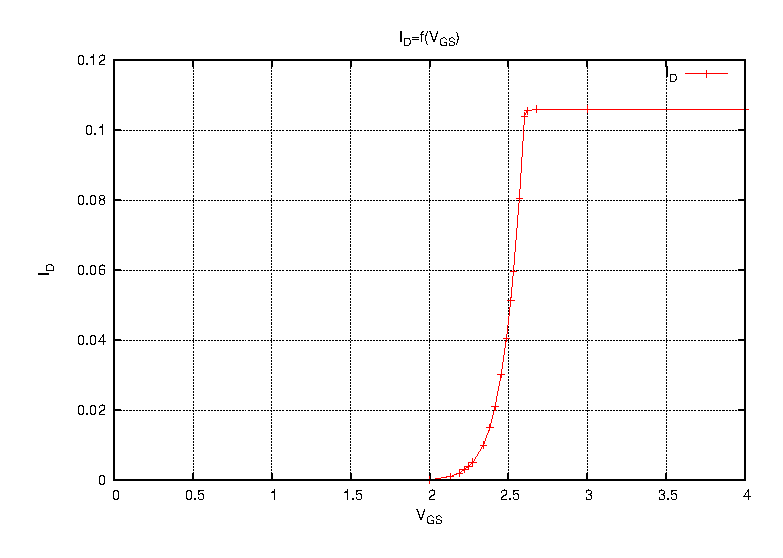
\includegraphics{mesures/id_vgs.eps}
\end{center}
}

\Question{
Cette caractéristique est-elle linéaire ? Dans quelle mesure cette source de courant commandée en tension est-elle utilisable pour amplifier ?
}
{
Non
}


\Question{
Choisir judicieusement un point de fonctionnement sur le relevé précédent. En utilisant le faisceau
 de courbes\footnote{\label{fn:datasheet}en utilisant les caractéristiques du transistor annexe
\ref{anx:mos_doc}} $I_D=f(V_D)@V_{GS}{=cte}$ et la droite de charge du transistor pour ce point de
fonctionnement, indiquer dans quelle zone fonctionne le transistor.

En déduire l'amplitude maximale possible en sortie pour le point de fonctionnement choisi.
\label{Q:Q9}
}{}


\section{Amplifier avec un montage en source commune}

La partie précédente permet de conclure que l'amplification est possible avec un transistor MOS. Nous allons donc construire un montage amplificateur autour du transistor.

La résistance sert à \og convertir \fg le courant qui circule dans le transistor en tension.

\begin{figure}[H]
%\vspace{-0.3cm}%dirty hack
	\begin{center}
		\begin{circuitikz}[scale=0.8]
		\draw
		(0,0) to [sV=$e(t)$] (0,2)
		(0,2) to [short] (1,2)
		(0,0) to (1,0)
		(1,2) to [open, v^<=$v_{in}$](1,0)
		(1,2) to [short,o-] (2,2)
		(1,0) to [short, o-] (2,0)
		(3,2) node[nigfete ] (mos) {}
		(mos.S) to [short] (3,0)
		(2,0) to (3,0)
		(mos.D) to [short](3,3) %, i<=$I_D$
		(3,3) to [R, l=$\SI{330}{\ohm}$] (3,5)
		(3,3) to [short, -o](4,3)
		(4,3) node[anchor=west] {$v_{out}$}
		(3,5) node[rground, yscale=-1] (alim) {}
		(alim.text) node {+12V}
		(3,0) node[ground] {}
		;\end{circuitikz}
	\end{center}
%\vspace{-0.7cm}%dirty hack
\caption{Montage à améliorer}
\label{fig:scidt}
\end{figure}

\Question{~
\begin{itemize}
    \item \label{Q:vout_th} Déterminer \textbf{théoriquement} \textsuperscript{\ref{fn:datasheet}} la forme du signal de sortie $v_{out}$ pour $$v_{in}=V_{max}\cdot \sin (2\pi \cdot f \cdot t)$$ avec $V_{max}=3V$, $V_{TH}\simeq 2.5V$ et $f=1000Hz$.
    \item Vérifier expérimentalement.
    \item Pourquoi ce circuit ne convient-il pas pour réaliser un amplificateur linéaire\footnote{Ce circuit convient par contre très bien à la commande en tout--ou--rien de circuit électriques de puissance ou à la réalisation de circuits logiques NMOS.} ? (2 éléments)
\end{itemize}
\label{Q:2elts1}
}
{
\begin{enumerate}
	\item le signal de sortie est écrêté et non linéaire
	\item sa moyenne est non nulle
\end{enumerate}
Le public manque généralement d'audiophiles et il faut leur expliquer que l'écrêtage change le contenu fréquentiel et que le HP ne supporte pas les tensions continues.
 % avec $U_{max}=2V$ et $\omega= 6283 rd/s$$Umax= V$ et $\omega=$.
\label{Q:2elts2}
Avec $R_D=330\Omega$ et $V_{max}=3V$ :
\begin{center}
	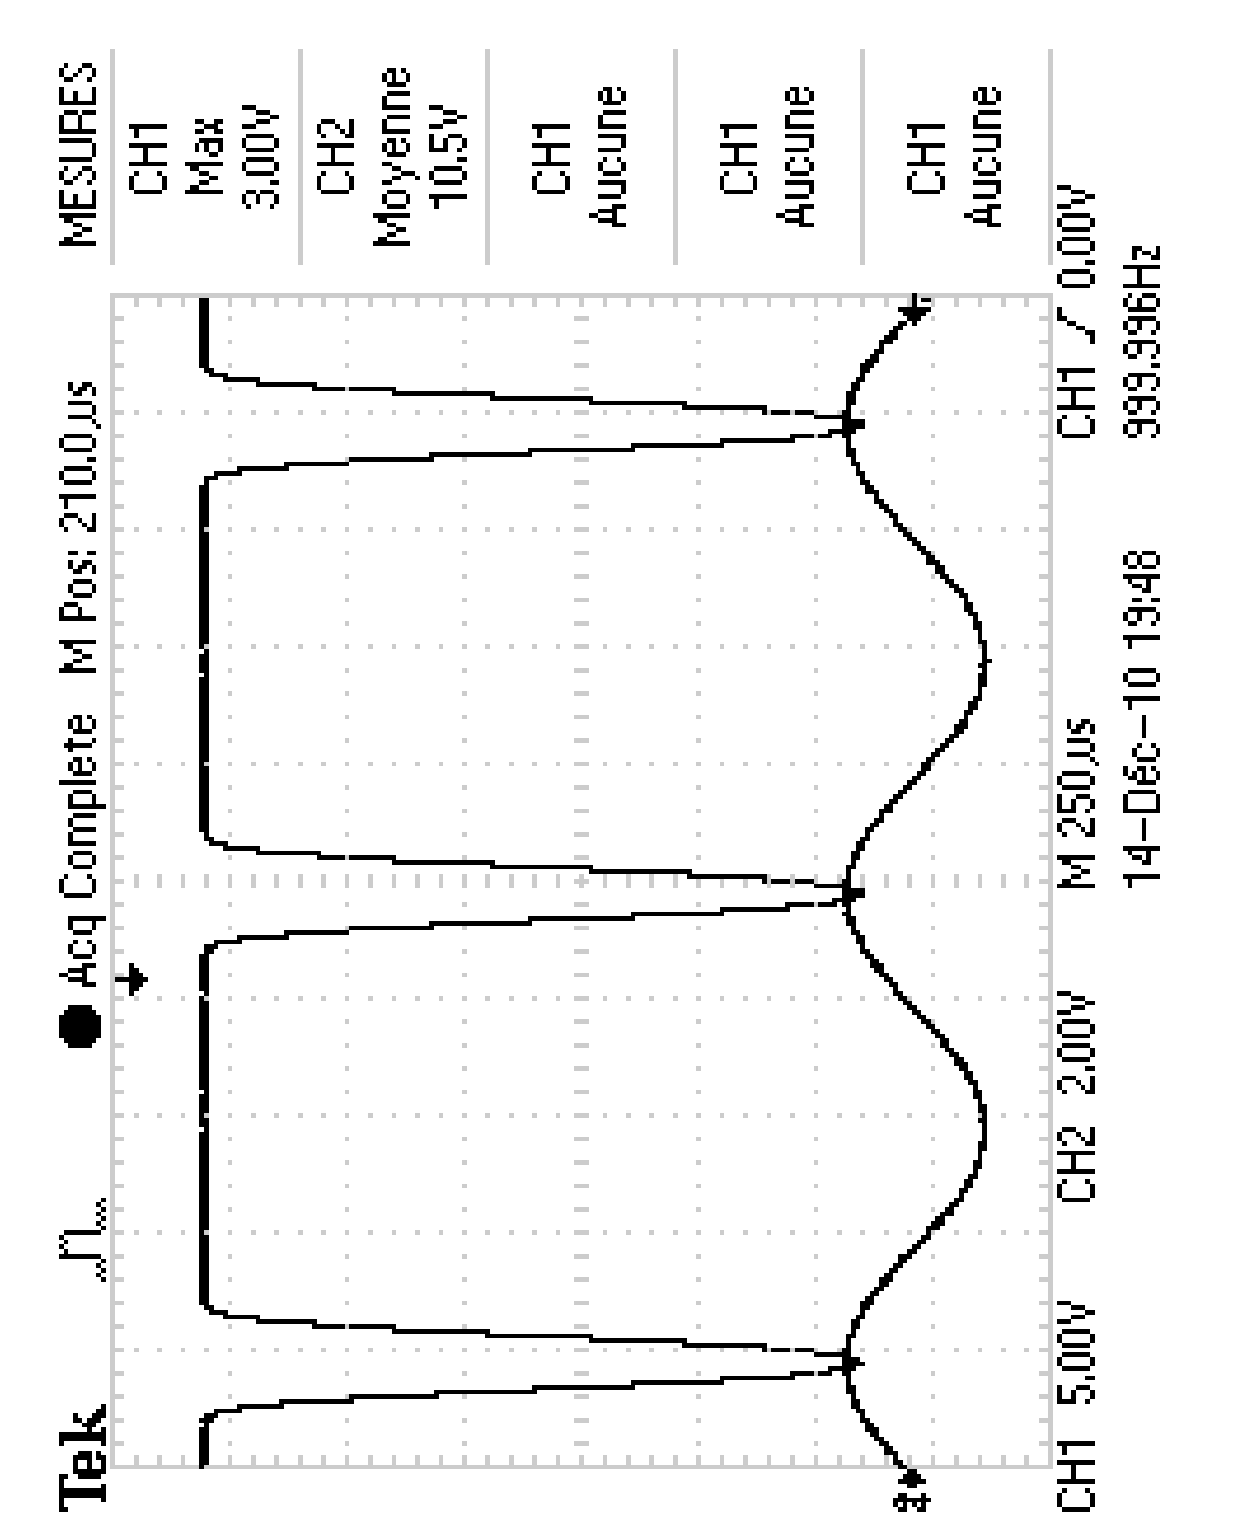
\includegraphics[angle=270, width=10 cm]{mesures/tek0002.eps}
\end{center}
}

\Question{~
\begin{itemize}
    \item Que faut-il faire pour corriger chacun des 2 problèmes ?
    \item Proposer une solution et vérifier expérimentalement (utiliser les possibilités du générateur).
\end{itemize}
}
{
%Cette question sera reformulée en "Que faut-il faire\dots ?" TODO
\begin{enumerate}
    \item Ajouter une composante continue pour se placer dans la zone de saturation $\Longrightarrow$ ajout d'une tension de polarisation
    \item Ajouter un filtre passe haut en sortie pour filtrer la composante continue
\end{enumerate}
}

\Question{~
\begin{itemize}
    \item \label{Q:capa_inout} Comment injecter un signal à moyenne nulle dans ce circuit en considérant les corrections apportées au circuit à la question précédente ?
    \item De même, que faire pour obtenir une tension de sortie à moyenne nulle ?
\end{itemize}
}
{%Et celle ci sera reformulée par "Comment faire\dots ?" TODO
On ajoute une capacité de découplage en entrée et en sortie et un pont résistif pour la polarisation
}

%NB : Généralement, la valeur de la composante continue est fixée par un pont résistif. %Dans le présent laboratoire, le pont résistif sera remplacé par un potentiomètre.


\Question{~
\begin{itemize}
    \item Tracer le schéma final de votre circuit corrigeant les deux éléments identifiés question \ref{Q:2elts1}. % et \ref{Q:2elts2}.
    \item Réaliser le montage correspondant.
\end{itemize}
}{
\begin{center}
		\begin{circuitikz}[scale=0.8]\draw
		(0,1) to [short,o-] (9,1)
		(4,6) to [short] (9,6)
		(0,3) node[anchor=east] {In} to [short,o-] (1,3)
		(0,3) to [open, v_=$V_{in}$]  (0,1)
		(1,3) to [C=$C_{in}$ ](1.5,3)
		(1.5,3) to [short,-*] (2,3)
%
		(2,6) node[european voltage source] (alim) {}
		(alim.text) node {$+V_{dc}$}
%
		(2,3) to [R, l_=$R_{b1}$](2,6)
		(2,3) to [R=$R_{b2}$](2,1)
%
		(4,3) node[nigfete] (mos) {}
		(mos.G) to [short] (2,3)
		(mos.D) to (4,4) to [R, l_=$R_D$] (4, 6)
		(mos.D) to [short,-*](4,3.5)  to [short] (4.25,3.5)
		(mos.S) to [short] (4,1)
		(4.25,3.5) to [C, l^=$C{out}$] (6,3.5) to  [short](6,3.5) to [short,-o](6.5,3.5)node [anchor=south] {Out}
		(6,3.5) to [generic, l_=$R_{ch}$] (6,1)
		(6.5,3.5) to [open,v^=$V_{out}$] (6.5,1)
		(9,1) to [battery, l_=$E$](9,6)
		;\end{circuitikz}
\end{center}
}

Les réponses aux questions \ref{Q:gain} à \ref{Q:pchg} doivent être étayées par des constations expérimentales.

\Question{~
\begin{itemize}
    \item Donner la relation entrée--sortie du montage et son gain. Préciser les limites de validité de la relation.
    \item Vérifier expérimentalement.
    \item Il %peut être judicieux
    vous est proposé d'utiliser le mode XY de l'oscilloscope.
    \item Indiquer  sur votre relevé les limites d'écrêtage et de linéarité, comparer avec le résultat de la question~\ref{Q:Q9}.
\end{itemize}

\label{Q:gain}
%
}
{
$$V_{ds}=-g_m\cdot R_D \cdot V_{in}$$

Bien que cette relation soit valable quelque-soit le régime de fonctionnement du transistor, seule la partie où le $g_m\neq 0$ est intéressante pour l'application.

Utilisation du mode XY :
mettre un signal triangulaire ($1kHz$, qqes V) à l'entrée du montage, afficher $V_{out}=f(V_{in})$ sur l'oscillo.

 Il peut être nécessaire de charger un peu la sortie avec une résistance.

Le mode XY permet de constater l'effet de la polarisation sur le gain et sur l'écrêtage du signal.

Avec $R_D=100\Omega$ :
\begin{center}
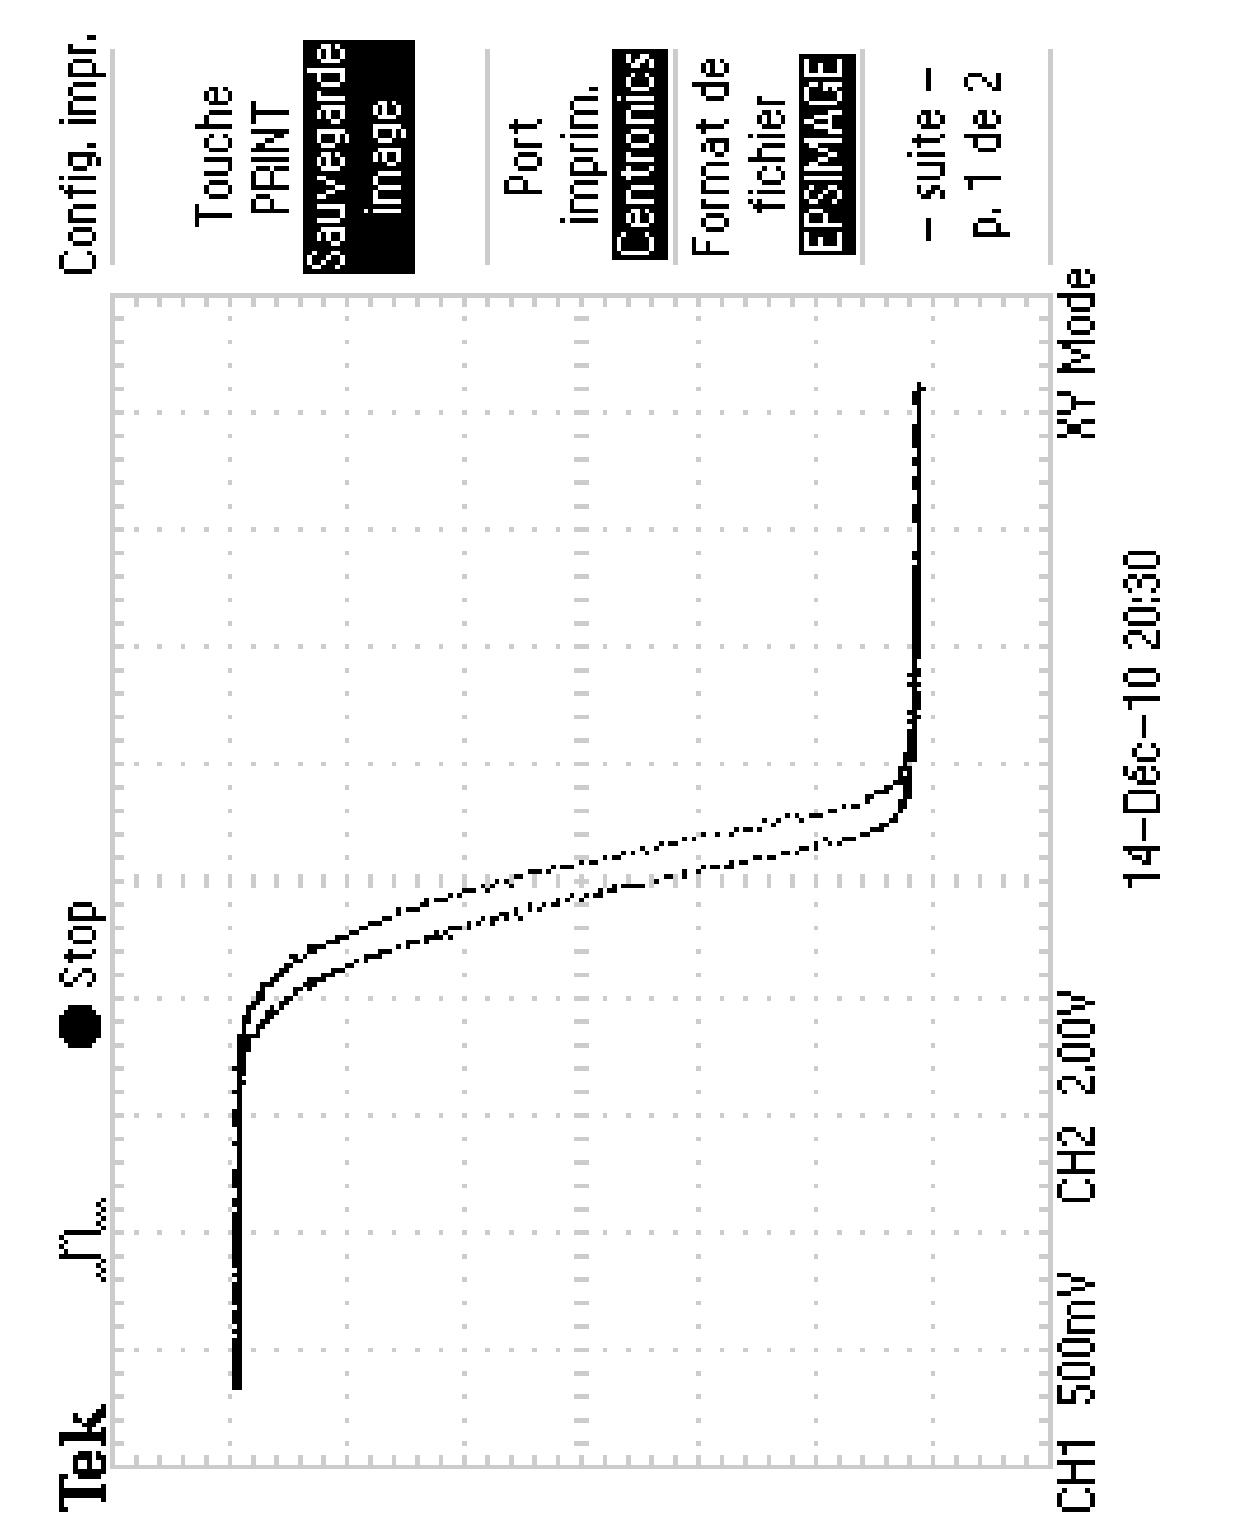
\includegraphics[angle=270, width=10 cm]{mesures/tek0004.eps}

\end{center}
}

\Question{~
\label{Q:PF}
\begin{itemize}
    \item Quelle est l'influence de la composante continue sur les caractéristiques du montage ?
    %\item Comparer à la source idéale.
    \item Quelle est la valeur de la composante continue qui maximise l'excursion en sortie ? Qui maximise le gain ? Avec quel inconvénient ?
\end{itemize}
}
{
Utiliser le potentiomètre pour modifier a polarisation. On constate le changement de gain sur le tracé XY précédent.

La polarisation est idéale si le point $(0,0)$ fait partie du relevé. En pratique, ce point est atteint si $V_D=E/2=6 V$. Ce point maximise l'excursion (tension) en sortie du montage. Il existe un autre point "optimal" : celui offrant le gain maximum. Celui ci se trouve vers la fin de la zone ohmique. (réponse à retravailler)

cette valeur doit être déterminée expérimentalement pour une valeur fixée de $v_{in}$. Elle dépend de $V_{in}$, $g_m$, $R_d$ et $V_{dc}$

Les 2 cas de la question précédente peuvent être considérés.
}

\Question{~
\begin{itemize}
    \item Quel est le gain en tension du montage pour cette valeur ?
    \item Que se passe-t-il si la résistance de drain $R_D$ change ?
    \item Que devient $g_m$ ?
    \item  La relation déterminée à la question \ref{Q:gain} est-elle remise en cause ?
\end{itemize}
}
{
mesure $\Longrightarrow$ gain en tension $\Longrightarrow $ valeur du $g_m$.

Si $R_D$ change, \textit{à priori} $I_D$ change aussi et $g_m$ également. La relation de la question \ref{Q:gain} n'est pas remise en cause si on considère $g_m$ non constant dans celle-ci.

Exemples :
\begin{center}
$R_D=100\Omega$ :
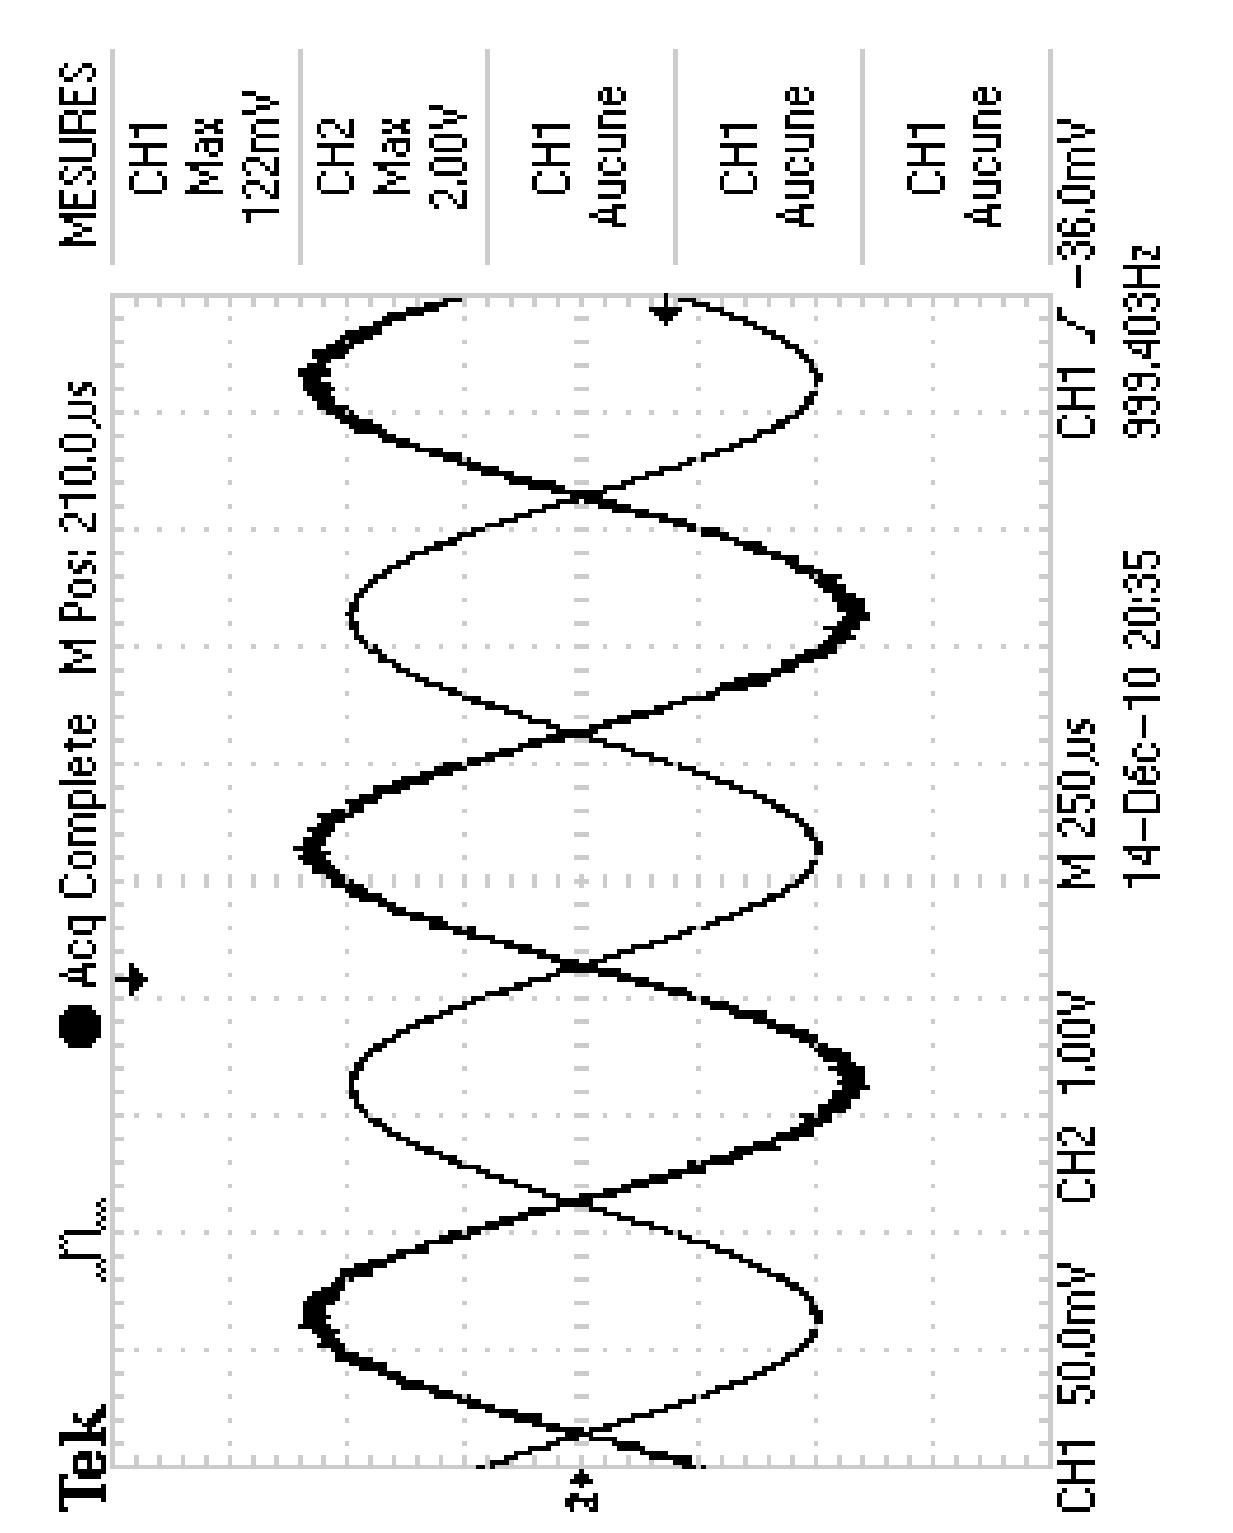
\includegraphics[angle=270, width=10cm]{mesures/tek0006.eps}

$R_D=330\Omega$ :
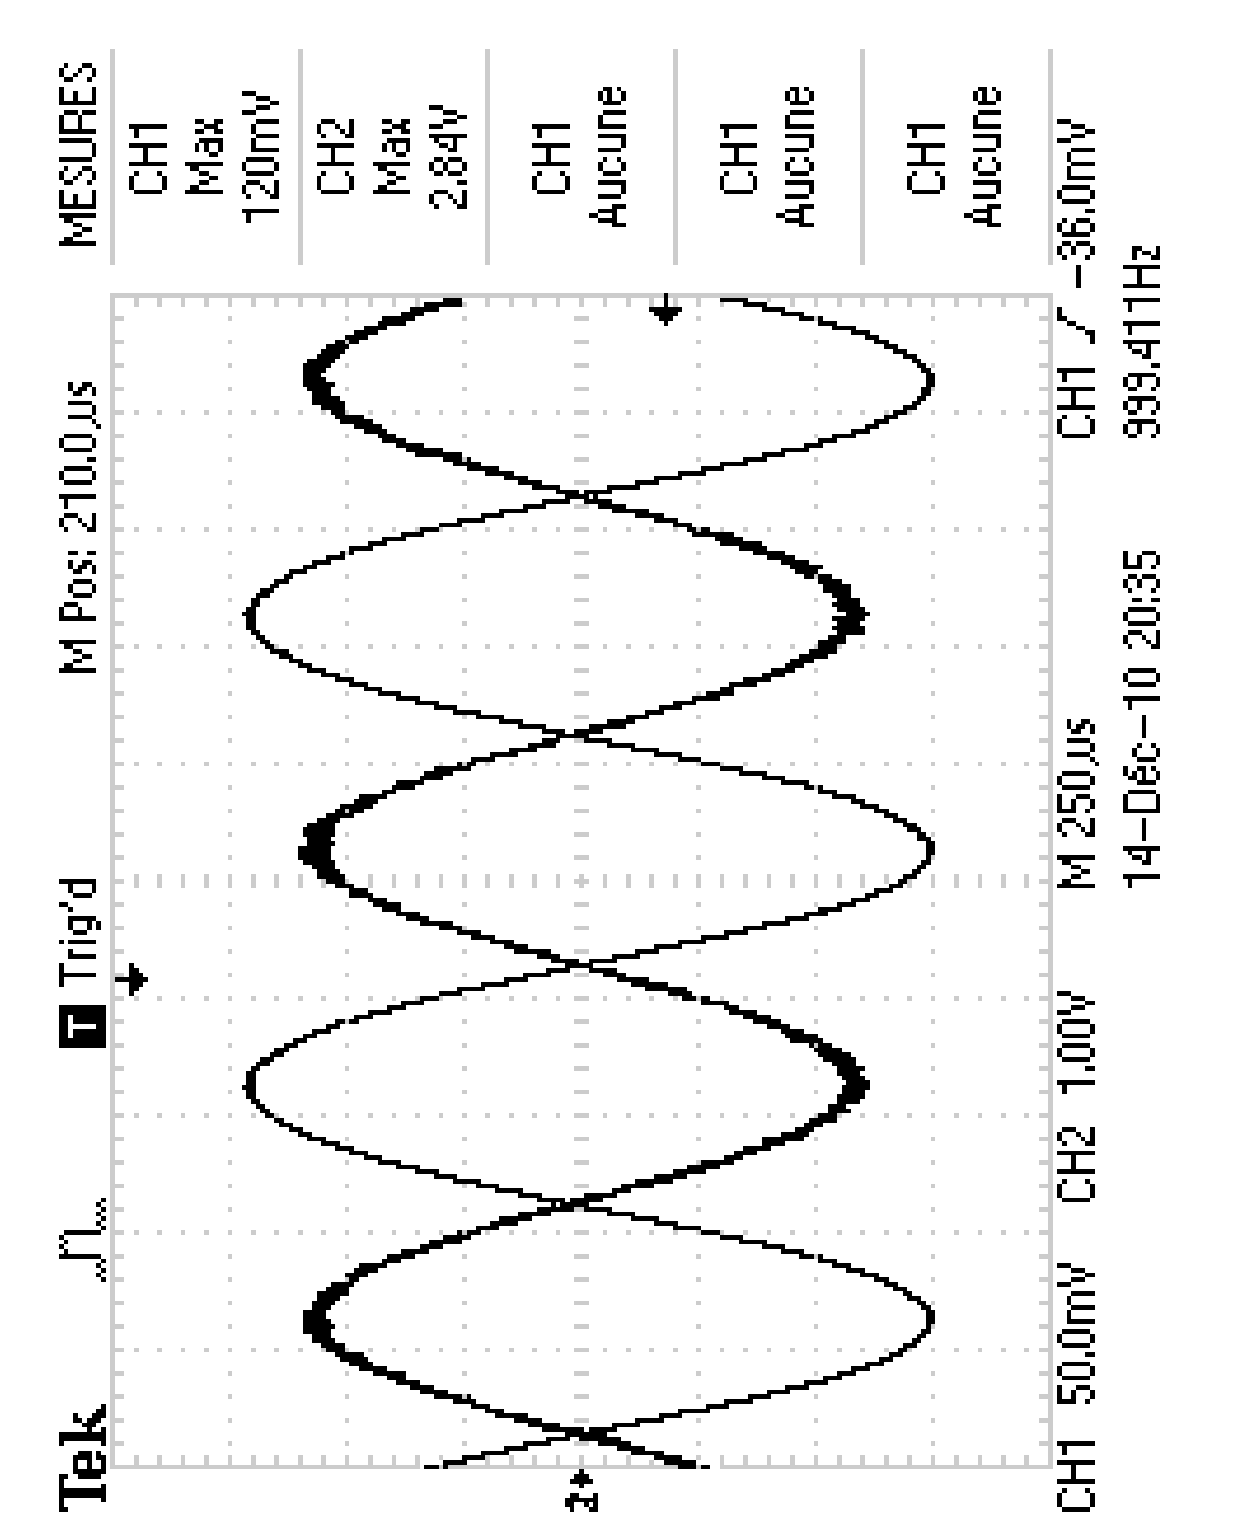
\includegraphics[angle=270, width=10cm]{mesures/tek0007.eps}

\end{center}
}

\Question{~
\begin{itemize}
\item  Que se passe-t-il si une charge est branchée en sortie ?
\item En utilisant un schéma à petit signal et des équivalences Thévenin--Norton, montrer que $\Delta V_{out}=f\left( R_{ch},\dots\right)$.
\item Vérifier expérimentalement avec $R_{ch}=330\Omega$ et $R_{ch}=100k\Omega$. Cet amplificateur peut-il être utilisé comme étage de puissance ? %est-il adapté à l'amplification audio ?
\end{itemize}

\label{Q:pchg}
}
{
Le gain diminue. Il suffit d'étudier le schéma petit signal pour s'en convaincre :
\begin{center}
	\begin{circuitikz}[scale=0.8]\draw
	(1,0) to [short,o-o] (11,0)
	(1,3) node[anchor=east] {In} to [short,o-] (1,3)
	(1,3) to [open, v_=$V_{in}$]  (1,0)
	(1,3) to [short] (3,3)
	(2,3) to [R, l_=$R_{b1}$](2,0)
	(3,3) to [R=$R_{b2}$](3,0)
	(3,3) to [short,-o](4,3) node [anchor=west] {}
	(4,3) to [open, v^=$V_{g}$](4,0)
	(6,3) to [cI=$g_m \cdot V_{g}$] (6,0)
	(8.5,0) to [R,l_=$R_D$] (8.5,3)
	(10,3) to [generic, l=$R_{ch}$] (10,0)

	(6,3) to [short,-o] (11,3) node [anchor=west] {Out}
	(11,3) to [open, v^=$V_{out}$](11,0)
	;\end{circuitikz}
\end{center}

Comme le gain dépend de la charge, cet étage n'est pas adapté à l'amplification de puissance.

Faire 2 tests : mettre $330\Omega$ et $100k\Omega$ en sortie.
}

\section{Synthèse -- dimensionnement d'un étage}
Cahier des charges :
\begin{itemize}
\item Bande passante : 20Hz--20kHz
\item Gain : 26dB
\item Amplitude de l'entrée : 0.1V, sinusoïdale, moyenne nulle
\item Tensions de sortie à moyenne nulle
\item Impédance d'entrée : $Z_{in}\geq10k\Omega$
\item Impédance de sortie : $Z_{out}\leq 1k\Omega$
\item Puissance statique dissipée par le transistor : $P_T\leq 0.5W$
\item Alimentation : $12V$ continue
\item Impédance de la charge : $Z_{ch}\geq 3.3k\Omega$
\end{itemize}
~\\

\Question{
\textit{Démarche proposée :}
\begin{enumerate}
\item Identifier les contraintes imposées par le cahier des charges.
\item Choisir la topologie de l'amplificateur (= schéma que vous avez obtenu en répondant aux questions précédentes).
\item Identifier les différents paramètres en fonction du cahier des charges (faire un schéma à petit signal).
\item Dimensionner les valeurs des différents composants du circuit sur base des courbes théoriques en annexe.
\item Déterminer la valeur de la tension de polarisation.
\item \textbf{Vérifier expérimentalement} en tenant compte des caractéristiques réelles de votre transistor. La polarisation devra être ajustée pour obtenir le bon gain.
%\item
\end{enumerate}
}
{
Voir corrigé annexe.

Gain de $26dB$ = $\pm 20$.

(Amplitude de sortie : $2V$ = on peut polariser à la bonne tension pour ajuster le gain)



$$V_s=-g_m\cdot \left( R_D//R_{ch} \right) \cdot V_{in}$$

→ $$-g_m\cdot \left( R_D//R_{ch}\right) =-20$$





La limite en puissance $P=V_{dc}\cdot I_D<=0.5W$ impose $I_D<=41.6mA$.

$V_{dc}=12V$ donc $g_m<=0.1S$.

On choisit de polariser au milieu de la droite de charge $V_D=6V$

donc $R_D>=146\Omega$

Il faut choisir $R_D$ tq l'influence de la charge soit faible sur le gain : $R_D<<R_{ch}$.

Si on choisit $R_D=330\Omega$,

on a $I_D=18mA$ → $g_m=0.06S$ → $A= 20$

donc en choisissant la bonne tension de polarisation pour avoir $I_D=18mA$ ou encore $V_s=6V$, on obtient le gain de $26dB$ voulu.

Le circuit consomme (en négligeant le pont de polarisation) : $P=V_{dc}\cdot I_D=0.216W$
}

\appendix
%\newgeometry{top=1 in, bottom=1 in, left=1 in, right=1 in} % Yeah, that's bad to play with margins
% \section{Le transistor NMOS}
%
% \label{anx:mos}
% Le transistor NMOS est un transistor MOS à canal N.
%
% Le symbole utilisé est visible figure \vref{fig:mos_elec2}.
% \begin{figure}[H]
% 	\begin{center}
% 		\begin{circuitikz}[scale=0.8] \draw
% 		(2.25,1) node[nigfete] (mos) {}
% 		(mos.D) -- (2.25,2) to  [short, -o](3.25,2)  node[anchor=west] {D}
%
% 		(mos.S) -- (2.25,0) to [short, -o](3.25,0)  node[anchor=west] {S}
%
% 		(2.25,0) to [short, -o](0,0)  node[anchor=east] {S}
%
% 		(0,2)  node[anchor=east]{G}[short,o-] to  (1,2) -- (1,1) -- (mos.G)
% 		;\end{circuitikz}
% 	\end{center}\vspace{-0.7cm}
% \caption{Symbole du transistor NMOS}
% \label{fig:mos_elec2}
% \end{figure}
% \vspace{-1cm}

%
% \subsection{Régimes de fonctionnement}
% Le transistor MOS est utilisable selon 3 régimes de fonctionnement.
%
% Le changement de régime est conditionné principalement par la valeur de $V_{GS}$.
% \subsubsection{Coupure}
% Pour $V_{GS}<V_{TH}$, $I_D=0$
% \subsubsection{Zone Ohmique ou triode}
% Pour $V_{GS}>V_{TH}$ et $V_{GD}>V_{TH}$, le transistor fonctionne en zone ohmique :
% $$I_D=\mu _0 C_{ox} \frac{W}{L}\left( V_{GS} - V_{TH}- \frac{V_{DS}}{2}\right)V_{DS} $$
% avec les constantes :
% \begin{itemize}
% \item [$\mu _0$] mobilité des porteurs
% \item [$C_{ox}$] capacité surfacique de l'oxyde de grille
% \item [$W$] largeur du canal
% \item [$L$] longueur du canal
% \item [$V_{TH}$] tension de seuil
% \end{itemize}

% \subsubsection{Zone de Saturation}
% Pour $V_{GS}>V_{TH}$ et $V_{GD}<V_{TH}$, le transistor fonctionne en zone saturée :
% $$I_D=\mu _0 C_{ox} \frac{W}{2L}\left( V_{GS} - V_{TH} \right) ^2 $$
%
% Puisque $V_D$ est absent de cette équation, $V_D$ n'influence pas $I_D$ : dans cette zone, le transistor se comporte donc comme une source de courant constante -- dont la valeur $I_D$ dépend néanmoins de $V_{GS}$ (voir figure \ref{fig:ps}).
% La transconductance $g_m$ ($[S]$) est définie pour ce modèle par : $$g_m=\frac{\partial I_D}{\partial V_{GS}}$$
%
% \begin{figure}[H]
% 	\begin{center}
% 		\begin{circuitikz}[scale=0.8]\draw
% 			(0,0) node[anchor=east] {G}
% 			to [short, o-] (1,0)
% 			to [open, v=$V_{GS}$] (1,-2)
% 			to [short, -o] (0,-2)
% 			to  (0,-2) node[anchor=east] {S}
% 			to [short] (3,-2)
% 			(3,0) to [cI=$ g_m \cdot V_{GS}$] (3,-2)
% 			(3,-2) to [short, -o] (4,-2) node[anchor=west] {S}
% 			(3,0) to [short, -o] (4,0)
% 			to node[anchor=west] {D} (4,0)
% 		;\end{circuitikz}
% 	\end{center}\vspace{-1cm}
% \caption{Schéma équivalent du transistor en zone de saturation}
% \label{fig:ps}
% \end{figure}
% \vspace{-1.2cm}

\section{Caractéristiques du transistor NMOS BS170}
\label{anx:mos_doc}
\begin{center}
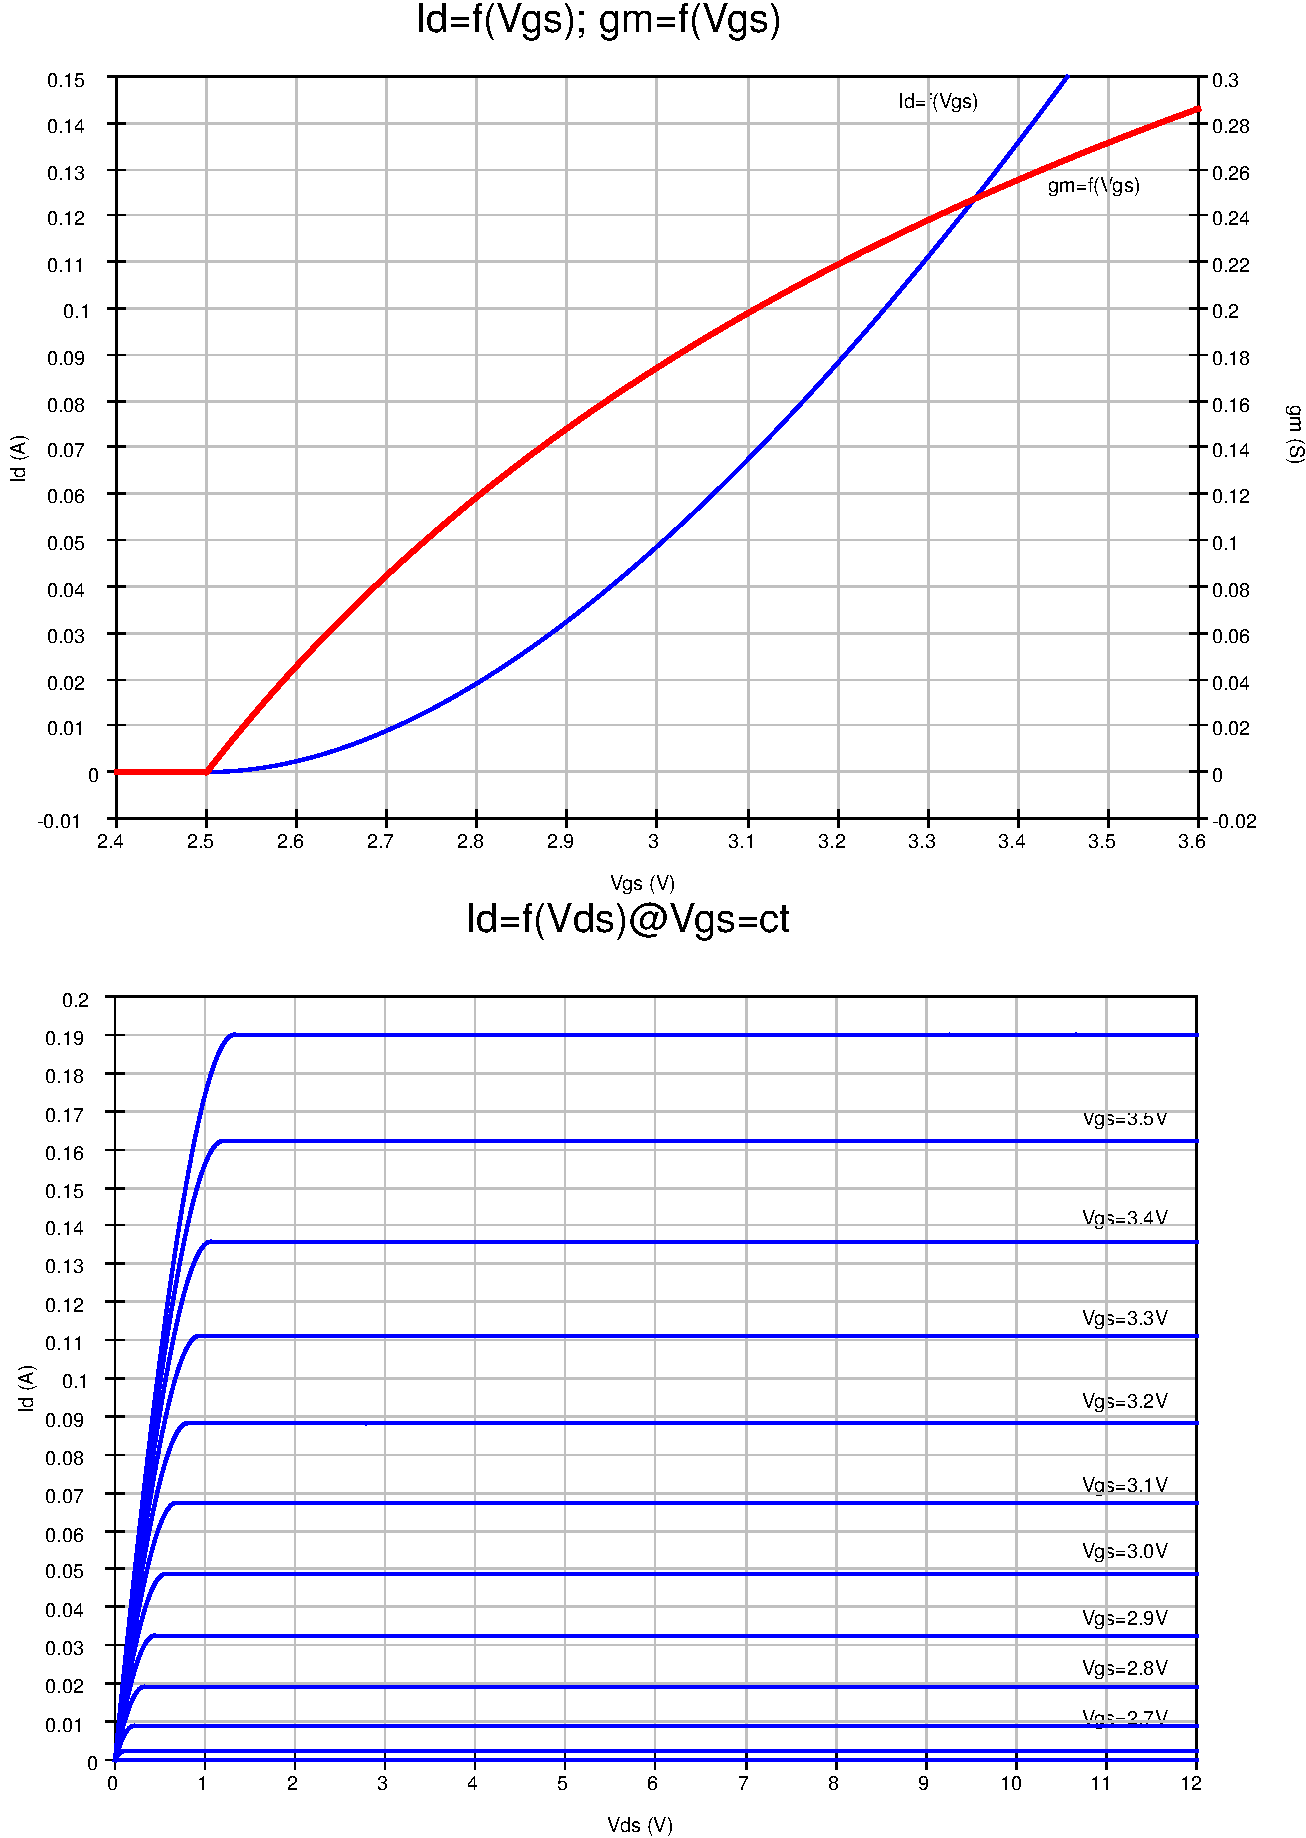
\includegraphics[width=16cm]{courbes_mos_2k16-crop.pdf}
% les courbes ici sont ont été corrigée et sont cohérentes.
\end{center}

\phantomsection
\addtocontents{toc}{
\href{http://pdf.datasheetcatalog.com/datasheets/70/123316_DS.pdf}
{\textbf{Documentation du transistor NMOS (lien cliquable)}}
{\attachfile[icon=Graph, color=0 0.75 1,description =Documentation du transistor NMOS BS 170 ]{./Documentation_BS170.pdf}}}

\label{anx:mos_datasheet}
%include pdf here
\end{document}
